\documentclass[11pt,twoside,a4paper]{article}

\usepackage{graphicx}
\usepackage[utf8]{inputenc}

\title{User Guide}
\author{Erik Brännström}
\date{December 16, 2012}

\begin{document}

\maketitle

\section{Introduction}

\begin{figure}[htb]
	\centering
	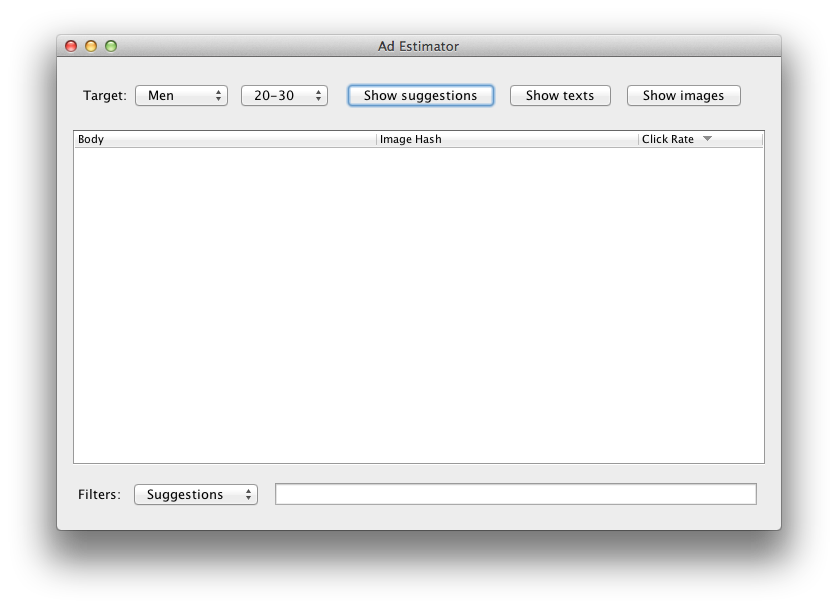
\includegraphics[width=1.0\textwidth]{gui-original.png}
	\caption{Application screenshot}
	\label{fig:GUI}
\end{figure}

The Ad Estimator was developed with the purpose of aiding marketing professionals in dealing with large amounts of data from marketing campaigns on Facebook. The perhaps most notable feature of the application is that it can automatically identify combinations of ad properties (e.g. text and image) which haven't been tested and estimate how well those new ads would perform.

Another useful feature is the property overview, where the user of the application can get a list of all property values used and their average performance. This can be used to for example quickly get an idea of which image is the most effective one.

All these functions can be limited to only present information for specific target groups, and the application also provides methods to filter information so that only what is relevant is shown.

\section{Knowledge bases}
Data is separated into knowledge bases, and they do not share any data between them. This is useful in order to separate different markets from each other, such as advertisement in different languages.

The application automatically creates a knowledge base called Default, but new knowledge bases can easily be created using the menu item New KB under the Knowledge bases menu. There is also an option to remove the currently active knowledge base. This will remove all data for that knowledge base and should thus be used with care.

When the user changes knowledge base, the targeting option are automatically updated to match that data. It also means that any reports that are imported from the File menu are stored in that knowledge base.

\section{Import and export}
As mentioned in the previous section, any reports that are imported will be stored in the active knowledge base, so make sure the correct one has been selected before importing.

The application currently only supports reports from Facebook. The reports can be downloaded from the Power Editor and must be in CSV format. The application only stores the information it requires and discards all other fields, so the application should not be considered as a backup system of sorts.

In order to facilitate importing ads back to Facebook, there is also an export function under the File menu. It exports the information from the rows that are currently selected in the table as well as the chosen targeting options. There is also an option to input a campaign name for the ads, but it can be left empty.

The export function uses a template to create the output file. The template is available in the resources folder and is named export-template.csv. Changing this file is not recommended unless you are a developer who have studied the technical documentation of the system.

The exported file is in CSV format and can be uploaded directly to the Power Editor.

\section{Targeting}
The application will automatically update the available values of the targeting properties when changing knowledge base, as well as update the values when a new report is imported in case new options are introduced.

The application currently supports targeting on gender and age, where the latter is actually the combination of the minimum and maximum age properties on Facebook. The matching is exact, so that for example selection age group 20-25 will only match that exact range and not for example 22-23, even though it is numerically contained in the larger group.

\section{Information views}
There are two possible views in the table. The full view is called so because it contains columns for all ad properties, where as the property view only has a single ad property column.

\subsection{Full view}
This view is shown when the Show suggestions button is pressed. It lists all ads in the current knowledge base that match the chosen targets and filters. It will also show the click rate or, in the case of suggested ads, the estimated click rate. Ads that are estimated will have a sand-colored background to differentiate them from the existing ads.

\subsection{Property view}
The property view is shown when clicking the Show texts or Show images buttons. The view will show the average click rate for all values of the chosen ad property. This view will never show any estimated ads.

\section{Filters}
In the bottom section of the application are two functions for filtering the data in the table. The selection box to the left is for filtering on the type of ad in the table. The possible values are Existing, which shows ads that have been run online; Suggestions, which are ads that have been created and estimated by the application; and All, which shows both types. Note that suggested ads have a non-white background color in order to make them stand out.

The text box to the right is a free text search field. This means that only rows that have at least one value which matches the text will be shown. This is useful to view ads with for example a specific image. The search is case-insensitive.

\end{document}